ACH is currently being used as the primary IPC method for the Primary Hubo Controller (PHC) for the Hubo2 Plus full-size humanoid robots.  
The Hubo2 Plus is a 130 $cm$ tall humanoid robot commonly referred to as Hubo.  
Hubo weighs 37 $kg$ and has 40 DOF.  
There are 12 DOF in each leg, roll, pitch and yaw in the hip, pitch in the knee and roll and pitch in the ankle.  

The PHC runs on the concept of using separate process for 

The primary PHC process is a daemon that talks over the CAN bus to all of the Hubo motor drivers and sensors.  
The \textit{feedforward} and \textit{feedback} states are stored in the \textit{HUBO\_REF\_CHANNEL} and \textit{HUBO\_STATE\_CHANNEL}.  
All information is stored in SI units.  The \textit{HUBO\_REF\_CHANNEL} holds a strut that has the desired reference for each of the joints in $rad$.  
The \textit{HUBO\_STATE\_CHANNEL} contains the sensor data and that joint status data.  T
his includes:

\begin{itemize}
                \item Encoder position (rad), at each joint
                \item IMU x angle (rad), at CoM
                \item IMU y angle (rad), at CoM
                \item IMU Vx velos(rad/sec), at CoM
                \item IMU Vy velos(rad/sec), at CoM
                \item FT Mx moment (Nm), in Feet
                \item FT My moment (Nm), in Feet
                \item FT Fz force (N), in Feet
                \item Angle from acc Ax (rad), in Feet
                \item Angle from acc Ay (rad), in Feet
                \item G-force acc Az (G), in Feet
\end{itemize}

The PHC daemon runs in real-time using the preempt-rt kernel.  
All sensors are polled and motor references are set at the system period.  
This period is currently set to 0.004 $sec$, $T_H$.  
This period is limited by the bandwidth of the CAN communications bus which is currently set to 1.0 $Mbps$.  
Currently there are two CAN channels with one controlling the upper body and one the lower body.  
The operation frequency can be increase if more CAN channels are added.  
The PHC system is designed for ease of adding communication busses.  

At the beginning of each cycle the new references are set to each actuator.  
After each cycle the state is updated with the new sensor data.

A separate process will subscribe to the \textit{feedforward} and \textit{feedback} channels and run it's own real-time loop.  
This can run, update reference and read the feedback channel at any desired frequency within the processor and IPCs capabilities.
The PHC will always take the most recent reference from the feedforward channel at the rising edge of it's clock cycle with the period of $T_H$.

\begin{figure}[thpb]
  \centering
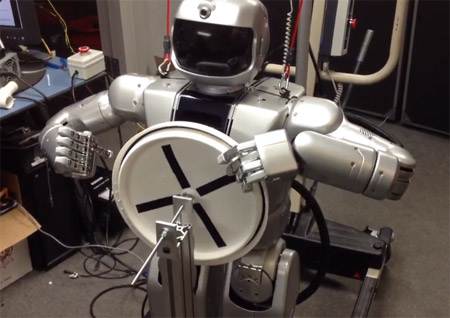
\includegraphics[width=1.0\columnwidth]{./pix/hubo_valve.png}
  \caption{Hubo running PHC turning a valve using trajectories created using Bi-RRTs. }
  \label{fig:valve}
\end{figure}

